%%---------------------------------------------------------------------------%%
%% Beamer ORNL Presentation Template
%%---------------------------------------------------------------------------%%

\documentclass{beamer}
%% The amssymb package provides various useful mathematical symbols
\usepackage{amssymb}
%% The amsthm package provides extended theorem environments
\usepackage{amsthm} \usepackage{amsmath} \usepackage{tmadd,tmath}
\usepackage{booktabs}
\usepackage{multirow}
\usepackage[compatibility=false]{caption}
\usepackage[labelformat=empty]{subcaption}
\usepackage{tikz}
\usepackage{ragged2e}

\usetikzlibrary{arrows}

%%---------------------------------------------------------------------------%%
%% THEME SETUP

\usetheme{CambridgeUS}
\usecolortheme{spruce}

%%---------------------------------------------------------------------------%%
%% SETUP STUFF
%%---------------------------------------------------------------------------%%

\logo{
\includegraphics[width=2cm]{new_logo}}

\setbeamercolor{item}{fg=MSUgreen}
\beamertemplatenavigationsymbolsempty
\setbeamertemplate{headline}{}
\setbeamertemplate{footline}{}
\setbeamertemplate{title page}
{
  \begin{tabular}{cr}
    \begin{minipage}{5.5cm}
      {\RaggedRight \bf \large \textcolor{MSUgreen}{\inserttitle}}\\
      \vspace{\baselineskip}\\
      \insertauthor\\
      \vspace{0.5\baselineskip}\\
      \insertinstitute\\
      \insertdate
    \end{minipage}
  \end{tabular}
}

\newlength{\DUtablewidth} % internal use in tables

%%---------------------------------------------------------------------------%%
%% TITLE

\title[MCREX]{Using Monte Carlo Algorithms to Achieve Resiliency \& Performance
  at Scale for Linear and Nonlinear Solver Applications}
\author{Thomas Evans \and Steven Hamilton}
\date[DOE, 2016]{DOE RX-Solvers \\ January 29, 2016}
\institute[ORNL]{Oak Ridge National Lab}

%%---------------------------------------------------------------------------%%
\begin{document}
%%---------------------------------------------------------------------------%%

{
  \usebackgroundtemplate{
    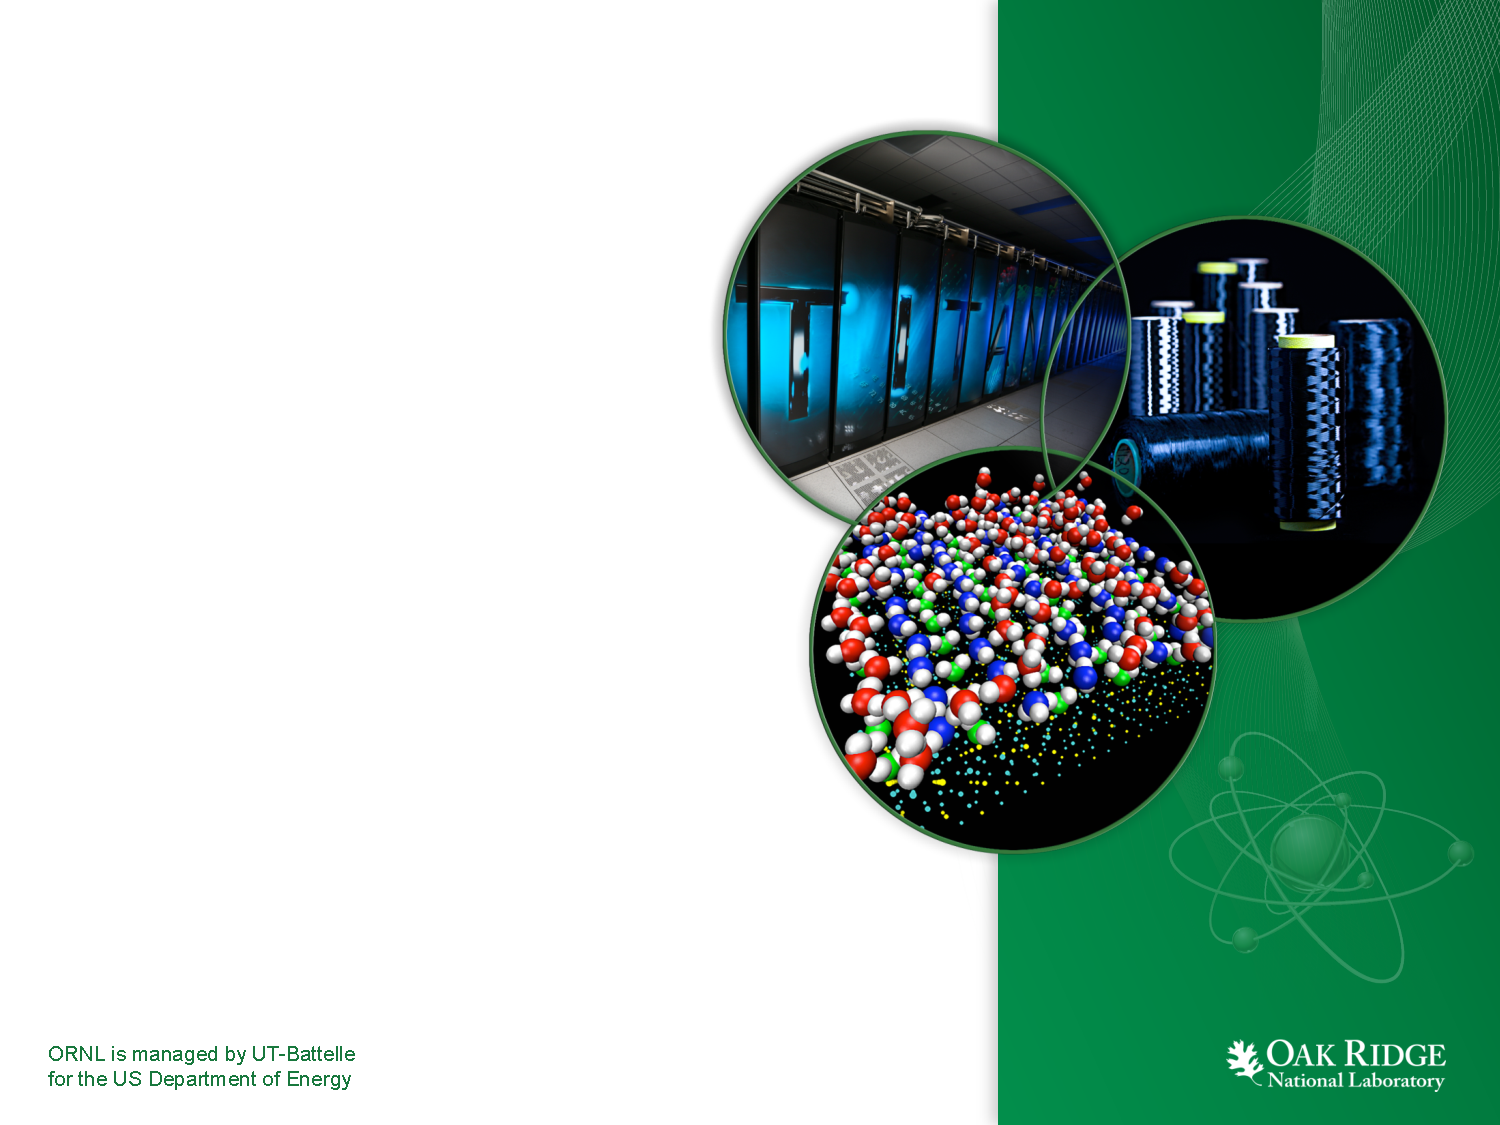
\includegraphics[width=\paperwidth,height=\paperheight]{title_template}}
  \setbeamertemplate{logo}{}
  \begin{frame}
    \titlepage
  \end{frame}
}

%%---------------------------------------------------------------------------%%
\section*{Outline}
%%---------------------------------------------------------------------------%%

\begin{frame}
  \tableofcontents[pausesections]
\end{frame}

%%---------------------------------------------------------------------------%%
\section{Project Status}
%%---------------------------------------------------------------------------%%
\subsection{Project Goals and Target Applications}
%%---------------------------------------------------------------------------%%

\begin{frame}{Project Objectives}

  The MCREX project has 3 objectives for the development of Monte Carlo solver
  methods for linear systems:
  \begin{itemize}
  \item Analyze and improve the iterative performance of Monte Carlo
    algorithms for linear systems
  \item Analyze and characterize the resilient aspects of Monte Carlo
    algorithms for linear systems
  \item Develop and model highly scalable parallel algorithms for the
    implementation of Monte Carlo algorithms for linear systems
 \end{itemize}
 The end goal is to develop a set of resilient, scalable algorithms for the
 solution of linear systems.  We have made significant progress in each of
 these areas as summarized below.

\end{frame}

%%---------------------------------------------------------------------------%%

\begin{frame}{Target Applications}

  \begin{itemize}

  \item Models defined by PDEs that result in sparse linear systems
    \begin{itemize}
    \item fluid flow
    \item radiation transport
    \item electrostatics
    \end{itemize}

  \item We have begun to analyze eigenvalue systems that are important in
    network systems analysis and data mining

  \item Much of our analysis work has used and idealized
    advection-diffusion-reaction system that has properties common to these
    application areas

  \item Extension to non-linear Navier-Stokes dropped due to budget
    constraints of funded proposal
  \end{itemize}

\end{frame}

%%---------------------------------------------------------------------------%%
\subsection{Overview and Status}
%%---------------------------------------------------------------------------%%

\begin{frame}{Monte Carlo for Linear Systems}
  \begin{itemize}
    \item Suppose we want to solve $\mathbf{Ax}=\mathbf{b}$
    \vfill
    \item If $\rho(\mathbf{I-A})<1$, we can write the solution using the
      Neumann series
      \begin{equation*}
        \mathbf{x} = \sum_{n=0}^{\infty} (\mathbf{I-A})^n \mathbf{b}
         = \sum_{n=0}^{\infty} \mathbf{H}^n \mathbf{b}
      \end{equation*}
      where $\mathbf{H} \equiv ( \mathbf{I-A} )$ is the Richardson
      iteration matrix
      \vfill
    \item Build the Neumann series stochastically
  \end{itemize}

  \[
  x_i = \sum_{k=0}^{\infty}\sum_{i_1}^{N}\sum_{i_2}^{N}\ldots
  \sum_{i_k}^{N}h_{i,i_1}h_{i_1,i_2}\ldots h_{i_{k-1},i_k}b_{i_k}
  \]

  \begin{itemize}
  \item Define a sequence of state transitions
  \end{itemize}
  \vspace*{-0.1in}
  \[
  \nu = i \rightarrow i_1 \rightarrow \cdots \rightarrow i_{k-1}
  \rightarrow i_{k}
  \]

\end{frame}

%%---------------------------------------------------------------------------%%

\begin{frame}{Solving the Heat Equation}

  \begin{figure}[h!]
    \begin{center}
      \includegraphics<1>[width=4in]{../NCState_seminar_2014/adjoint_1}
      \includegraphics<2>[width=4in]{../NCState_seminar_2014/adjoint_10}
      \includegraphics<3>[width=4in]{../NCState_seminar_2014/adjoint_100}
      \includegraphics<4>[width=4in]{../NCState_seminar_2014/adjoint_1000}
      \includegraphics<5>[width=4in]{../NCState_seminar_2014/adjoint_10000}
      \includegraphics<6>[width=4in]{../NCState_seminar_2014/adjoint_100000}
      \includegraphics<7>[width=4in]{../NCState_seminar_2014/adjoint_1000000}
      \includegraphics<8>[width=4in]{../NCState_seminar_2014/adjoint_10000000}
    \end{center}
    \caption{
      \only<1>{\textbf{Adjoint solution.}
        \textit{\sn{1}{0} total histories.} }
      \only<2>{\textbf{Adjoint solution.}
        \textit{\sn{1}{1} total histories.} }
      \only<3>{\textbf{Adjoint solution.}
        \textit{\sn{1}{2} total histories.} }
      \only<4>{\textbf{Adjoint solution.}
        \textit{\sn{1}{3} total histories.} }
      \only<5>{\textbf{Adjoint solution.}
        \textit{\sn{1}{4} total histories.} }
      \only<6>{\textbf{Adjoint solution.}
        \textit{\sn{1}{5} total histories.} }
      \only<7>{\textbf{Adjoint solution.}
        \textit{\sn{1}{6} total histories.} }
      \only<8>{\textbf{Adjoint solution.}
        \textit{\sn{1}{7} total histories.} }
    }
  \end{figure}
\end{frame}

%%---------------------------------------------------------------------------%%

\begin{frame}{Limitations of Monte Carlo}
  \begin{itemize}
  \item Solving linear systems of equations with ``pure'' Monte Carlo methods
    is generally intractable
    \begin{itemize}
    \item Central limit theorem is barrier to accurate solutions
    \end{itemize}
    \begin{figure}
      \centering
      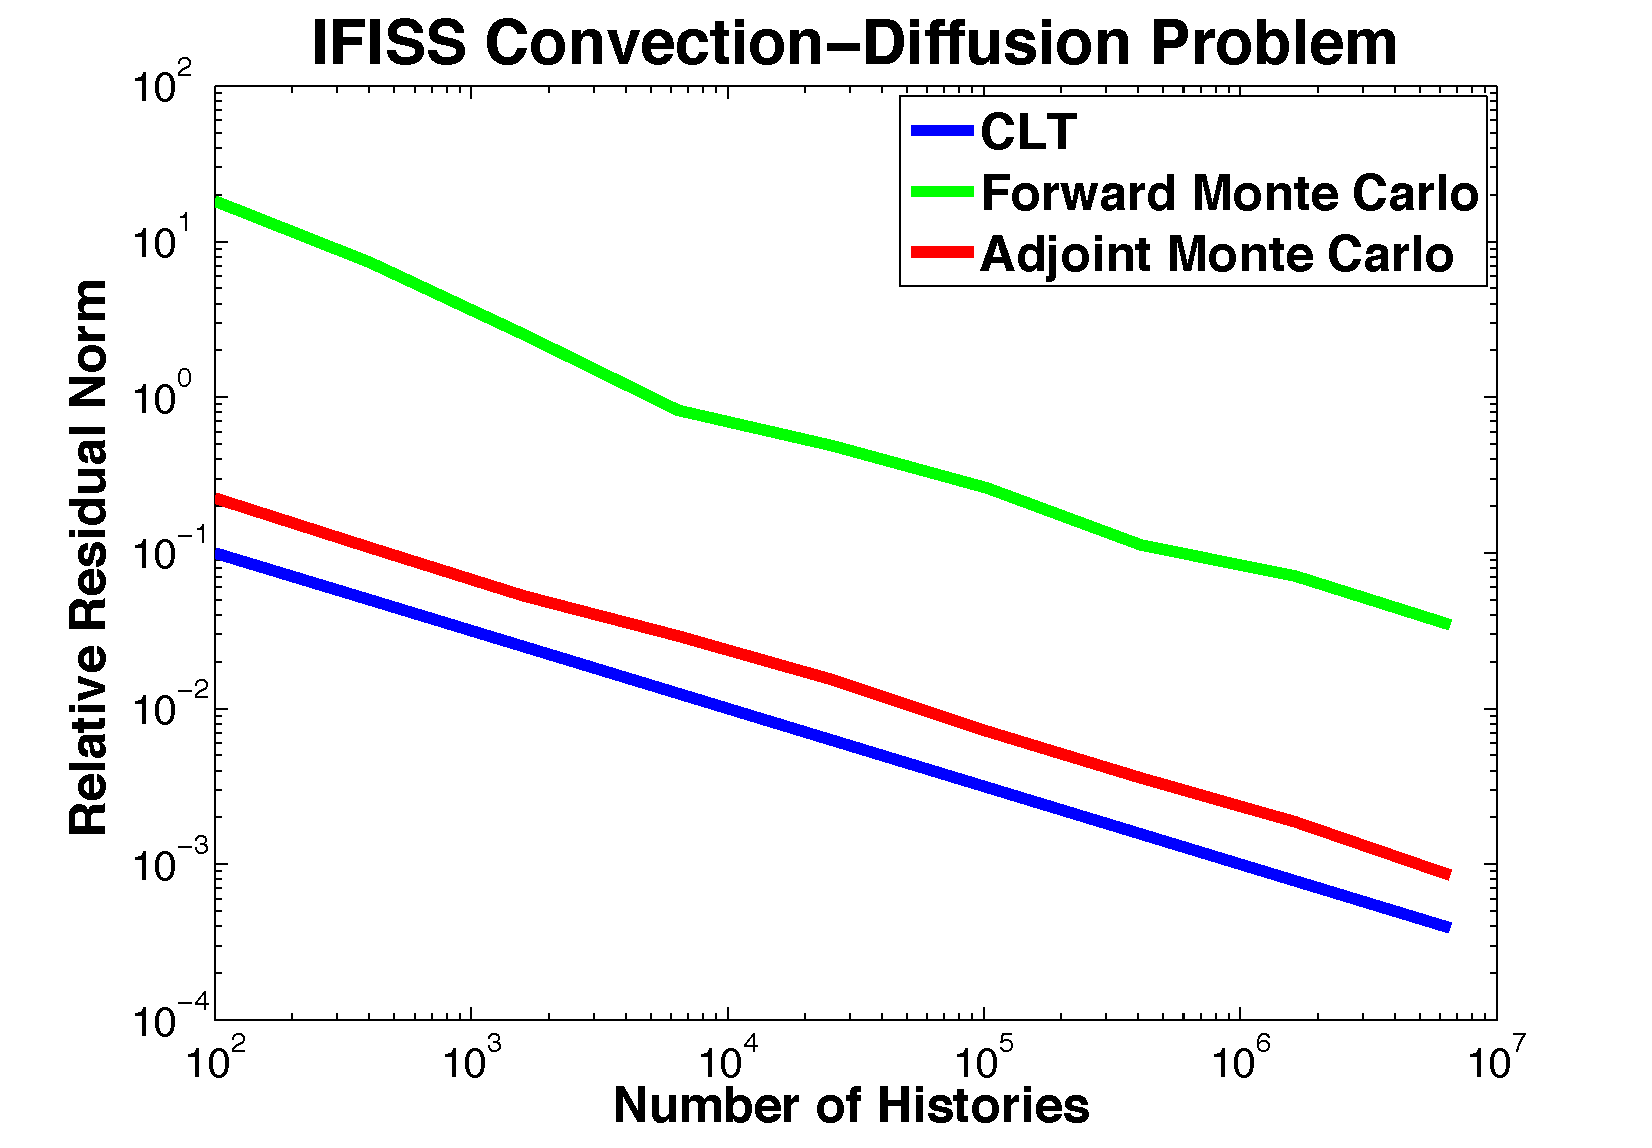
\includegraphics[width=1.75in]{../NCState_seminar_2014/Ifiss_ConvDiff}
    \end{figure}
  \item There is a potentially restrictive limit on the spectral properties of
    $\mathbf{H}$
    \begin{equation}
      \rho(\mathbf{H}) < 1\:, \rho(\hat{\mathbf{H}}) < 1\:, \hat{H}_{ij} =
      \frac{H_{ij}^2}{P_{ij}}
    \end{equation}
  \end{itemize}
\end{frame}

%%---------------------------------------------------------------------------%%

\begin{frame}{Monte Carlo Synthetic Acceleration}
  \begin{itemize}
  \item Address issue of convergence constrained by CLF
    \vfill
  \item Can be abstracted as a general linear solver
    \vfill
  \item Combine with Richardson iteration as a ``smoother'' in between
    Monte Carlo steps:
    \begin{align*}
      \mathbf{r}^k &= \mathbf{b} - \mathbf{Ax}^k \\
      \mathbf{x}^{k+1/2} &= \mathbf{x}^k + \mathbf{r}^k \\
      \mathbf{r}^{k+1/2} &= \mathbf{b} - \mathbf{Ax}^{k+1/2} \\
      \hat{\mathbf{A}} \mathbf{\delta} &= \mathbf{r}^{k+1/2} \\
      \mathbf{x}^{k+1} &= \mathbf{x}^{k+1/2} + \delta
    \end{align*}
  \item We still must address issue of convergence constraint by spectral radius
  \end{itemize}
\end{frame}

%%---------------------------------------------------------------------------%%

\begin{frame}{Preconditioned MCSA}
\vspace*{-0.2in}
  {
    \small
    \[
    \ve{r}^{k} = \ve{M}_L^{-1}(\ve{b}-\ve{A}\ve{M}_R^{-1}\ve{x}^{k})
    \]
    \[
    \ve{x}^{k+1/2} = \ve{x}^k + \ve{r}^k
    \]
    \[
    \ve{r}^{k+1/2} = \ve{M}_L^{-1}(\ve{b}-\ve{A}\ve{M}_R^{-1}\ve{x}^{k+1/2})
    \]
    \[
    \ve{M}_L^{-1}\ve{A}\ve{M}_R^{-1}\delta\ve{x}^{k+1/2} = \ve{r}^{k+1/2}
    \]
    \[
    \ve{x}^{k+1} = \ve{x}^{k+1/2} + \delta \ve{x}^{k+1/2}
    \]
  }
  \vspace*{-0.1in}
  \begin{itemize}
    \item Requires explicit construction of preconditioned matrix
      \begin{itemize}
        \item This has generally limited preconditioner selection to diagonal,
          block diagonal, sparse approximate inverse approaches
      \end{itemize}
    \vfill
    \item Sparsity in $\mathbf{A}$, $\mathbf{M}$, does not imply sparsity
      in $\mathbf{M^{-1}A}$
    \vfill
    \item Need to investigate preconditioning strategies that lead to sparse
      preconditioned systems
  \end{itemize}
\end{frame}

%%---------------------------------------------------------------------------%%

\begin{frame}{Monte Carlo as Approximate Polynomial Preconditioning}
  \begin{itemize}
    \item Using history length cutoff, Monte Carlo process is approximating
      a fixed length Neumann series polynomial
      \[
      x_i = \sum_{k=0}^{\infty}\sum_{i_1}^{N}\sum_{i_2}^{N}\ldots
      \sum_{i_k}^{N}h_{i,i_1}h_{i_1,i_2}\ldots h_{i_{k-1},i_k}b_{i_k}
      \]
    \vfill
    \item As number of histories grows, iteration count becomes identical to
      using ``true'' polynomial
    \vfill
    \item Why limit ourselves to the Neumann series polynomial?
      \begin{itemize}
        \item Chebyshev or GMRES polynomials are viable alternatives
      \end{itemize}
  \end{itemize}
\end{frame}

%%---------------------------------------------------------------------------%%

\begin{frame}{Neumann Series Polynomial}
  \begin{table}
    \caption{Adjoint MCSA with Neumann Polynomial, $1000 \times 1000$ Shifted Laplacian Matrix.
      Values are MCSA iteration counts (timing in milliseconds)
      \label{tab:lap_adjoint_neumann}}
    \centering
    \begin{tabular}{cccc}
      \toprule
      Histories per & \multicolumn{3}{c}{Polynomial Order} \\
      \cmidrule(lr){2-4}
      Iteration & 2 & 4 & 6 \\
      \midrule
      250 &  775(100) & 651(96) & 664(110) \\
      500 &  725(122) & 502(104) & 394(95) \\
      1000 & 707(174) & 482(179) & 366(144) \\
      2000 & 703(280) & 471(259) & 356(251) \\
      4000 & 698(494) & 467(497) & 350(458) \\
      8000 & 697(923) & 464(905) & 350(873) \\
      16000 & 695(1796) & 462(1768) & 347(1711) \\
      \bottomrule
    \end{tabular}
  \end{table}
\end{frame}

%%---------------------------------------------------------------------------%%

\begin{frame}{Chebyshev Polynomial}
  \begin{table}
    \caption{Adjoint MCSA with Chebyshev Polynomial, $1000 \times 1000$ Shifted Laplacian Matrix.
      Values are MCSA iteration counts (timing in milliseconds)
      \label{tab:lap_adjoint_cheby}}
    \centering
    \begin{tabular}{cccc}
      \toprule
      Histories per & \multicolumn{3}{c}{Polynomial Order} \\
      \cmidrule(lr){2-4}
      Iteration & 1 & 2 & 3 \\
      \midrule
      250 & - & - & - \\
      500 & - & - & - \\
      1000 & - & - & - \\
      2000 & - & 328(134) & - \\
      4000 & - & 296(210) & - \\
      8000 & - & 288(380) & 262(423) \\
      16000 & 1132(1866) & 283(721) & 175(550) \\
      \bottomrule
    \end{tabular}
  \end{table}
\end{frame}

%%---------------------------------------------------------------------------%%

\begin{frame}{Polynomial Methods -- Summary}
  \begin{itemize}
    \item Using history length cutoff rather than weight cutoff can lead to
      large reductions in iteration counts
      \vfill
    \item A good approximation to a few terms in the Neumann series
      performs better than a statistically noisy approximation to
      full series
      \vfill
    \item Significant reduction in iteration counts are possible using
      alternate polynomials, but generally outweighed by increase in number
      of histories required
      \begin{itemize}
        \item May be very beneficial from resiliency and parallel efficiency
          standpoints
        \item Will be re-evaluated in future efforts
      \end{itemize}
  \end{itemize}
\end{frame}

%%---------------------------------------------------------------------------%%

\begin{frame}{Sparse Approximate Inverse Preconditioning}



\end{frame}

%%---------------------------------------------------------------------------%%
\subsection{Software}
%%---------------------------------------------------------------------------%%

\begin{frame}{MCSA Implementations}

  \begin{itemize}
  \item {\bf MCLS} (\underline{github.com/sslattery/MCLS})
    \begin{itemize}
    \item Massively parallel (MPI) implementation of domain decomposed MCSA
      algorithm
    \item Implemented in Trilinos framework and callable through Trilinos'
      abstract numerical algorithms (Thyra, Stratimikos) interface
    \item Works with any Tpetra row matrix
    \end{itemize}
  \item {\bf Alea} (\underline{github.com/ORNL-CEES/Profugus})
    \begin{itemize}
    \item GPU-accelerated on-node MC solve
    \item Domain-local MC solves implemented for distributed systems as an
      additive Schwartz method
    \end{itemize}
  \end{itemize}

\end{frame}

%%---------------------------------------------------------------------------%%
\section{Transition and Roadmap}
%%---------------------------------------------------------------------------%%



%%---------------------------------------------------------------------------%%

\begin{frame}
\vfill
\centering
\huge Questions?
\vfill
\end{frame}

%%---------------------------------------------------------------------------%%
\end{document}
%%---------------------------------------------------------------------------%%

%%---------------------------------------------------------------------------%%
%% end of pres.tex
%%---------------------------------------------------------------------------%%
